As already anticipated in the summary, the present thesis implements a supervised learning model for music classification. This chapter will cover the technical basis necessary to have a sound understanding of the model, following the mindmap provided in figure \ref{fig:mindmap}.

\begin{figure}[h]
  \hspace*{-0.6cm}
  \centering
  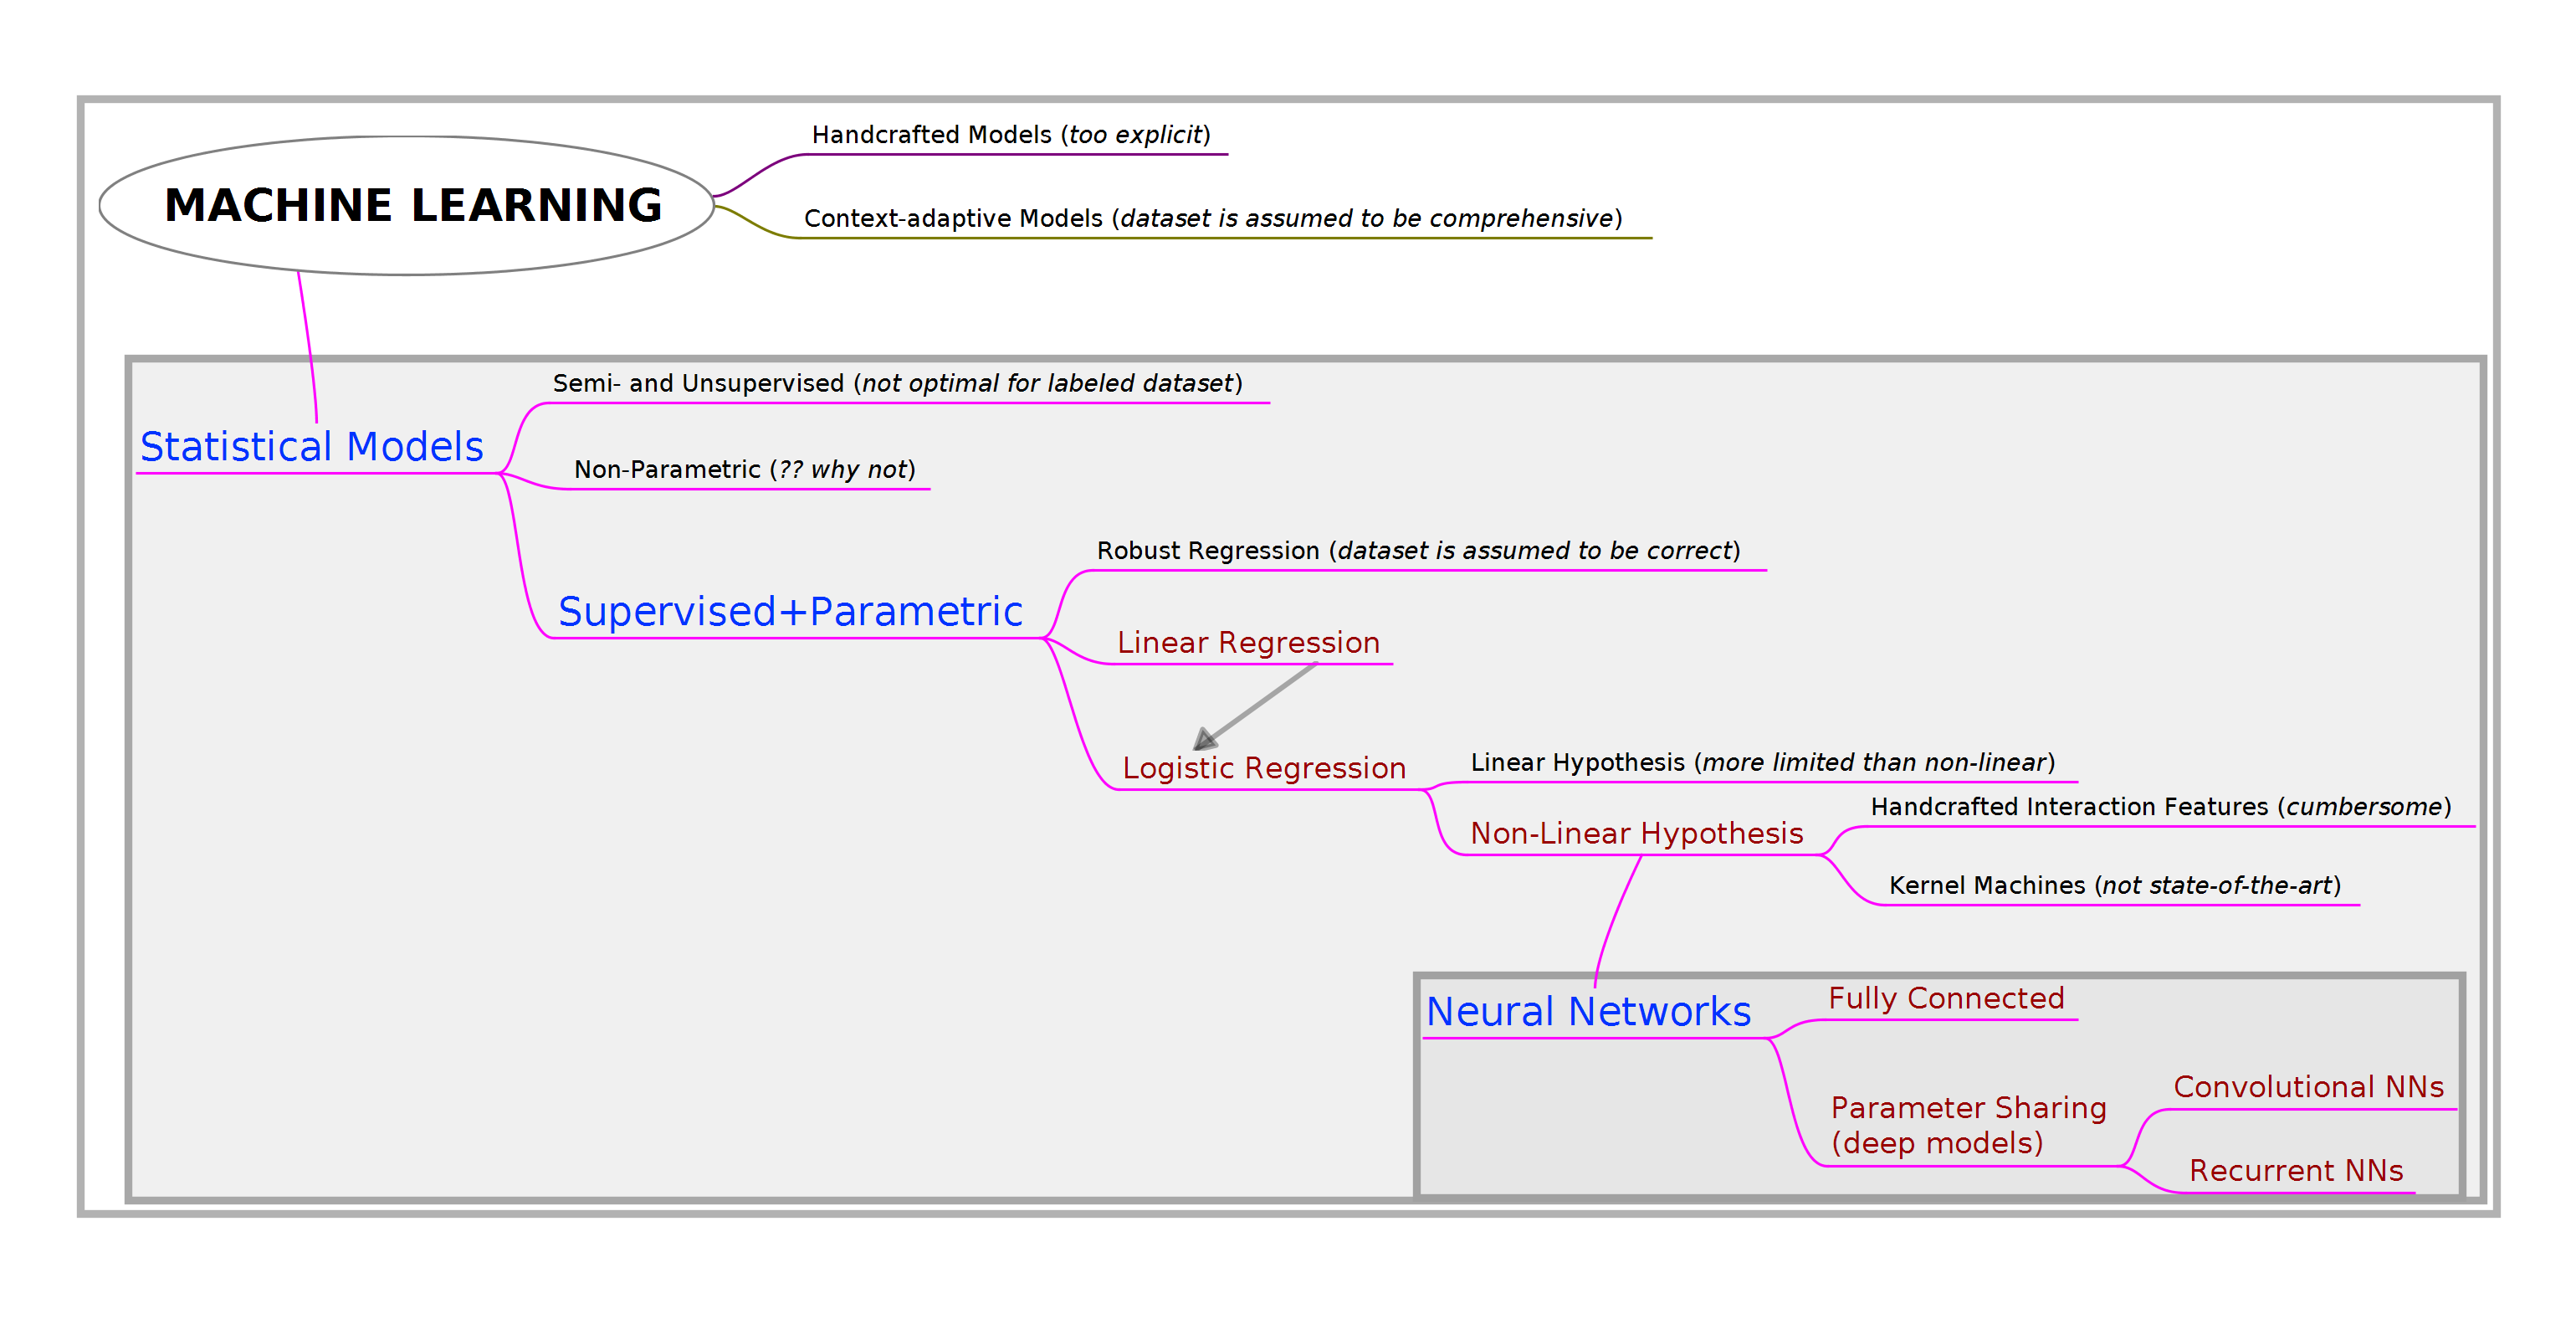
\includegraphics[scale=0.6]{freeplane/machine_learning.png}
  \caption{A mindmap of this chapter's contents. The concepts in the smallest font weren't used in this project, and are covered just enough to understand why (a small explanation can be found in the parentheses).}
  \label{fig:mindmap}
\end{figure}


The mindmap covers some machine learning models, building up from very simple mathematical concepts to the state of the art models for classification. But although deep learning is a specific kind of machine learning\cite[p. 98]{goodfellow}, it doesn't mention the word deep, for a reason: When a machine learning model is structured in hierarchical layers (like neural networks), it is possible to talk about its {\it depth}. In this context, {\it deep} learning models (as opposed to {\it shallow} models) are machine learning models with many layers. But the fact is that ``there is no single correct value for the depth of an architecture, nor is there a consensus about how much depth does a model require to qualify as {\it deep}''\cite[p.8]{goodfellow}. Also, it is much more reasonable to structure the chapter contents based on the mathematical techniques that the different models are based on, rather the exact number of implemented layers.\\


In fact, the depth of the model plays a very relevant role not only from a technical point of view, and there is much support to claim that ``Deeper models tend to perform better''\cite[p.202]{goodfellow}. The concept of {\it deep learning} is fairly new, dating from 2006\cite[p.13]{goodfellow}, but the practice has actually decades of rich history (there are many divulgative texts covering the history of deep learning in further detail, notably \cite{deephist} and also \cite[p.13]{goodfellow}).\\



\section{Machine Learning}

The main idea of machine learning was already formulated by Turing in 1950, with the idea of the {\it child programme} and the education process\cite{turing:50}: based on this idea, some steps in the solving process are automatically inducted from a given dataset instead of hardcoded. But this definition is very broad, and encompasses well over 60 years of history (some core techniques like the {\it least squares optimization} trace back to Gauss' times\cite{lso}), covering a wide amount of paradigms, structures, techniques and concepts used in many different applications. Tom M. Mitchell provided in 1997 a much more specific concept of learning applied to machines\cite[p.99]{goodfellow}:
\begin{quote}
  A computer program is said to learn from experience E with respect to some class of tasks T and performance measure P , if its performance at tasks in T , as measured by P ,improves with experience E.
\end{quote}
The advantage of this definition is that it involves a fairly simple set of elements, and expresses the rather complex task of learning as a relationship among them that not only is conceptually very elegant, but also very practical. It also seems to be widely accepted, being directly used in \cite{goodfellow} and \cite{coursera-ml}, and indirectly in \cite{russell}. But the fact is that it still encompasses a very broad range of AI techniques. John Launchbury, a director of the {\it Defense Advanced Research Projects Agency} (DARPA) has released very recently a brief Perspective on Artificial Intelligence\cite{darpa-slides}-\cite{darpa-vid}, in which he provides a more comprehensive and structured view. In it, he defines artificial intelligence as the ``{\it programmed} ability to process information'', that can be decomposed in a set of four skills: \textbf{perceiving}, \textbf{learning}, \textbf{abstracting} and \textbf{reasoning}. Based on this, he distinguishes 3 historical ``waves of AI'':
\begin{enumerate}
\item Handcrafted Knowledge (characteristical task: {\it describe}): ``Engineers create sets of rules to represent knowledge in well-defined domains. The structure of knowledge is defined by humans, the specifics are explored by the machine''. An example of this are the classical Chess AIs. This models have high capacity of reasoning, a minimal perceiving of the environment, and no learning or abstracting capability.
\item Statistical Learning (characteristical task: {\it categorize}): ``Engineers create statistical models for specific problem domains and train them on big data.''. In some cases, it is very difficult or impractical for humans to define a problem domain as an explicit set of rules, but much easier to collect a set of examples that implicitly responds to those rules. This kind of models are able then to learn an explicit representation of those rules by inspecting the dataset (ref manifold): as opposed to the deductive nature of the first-wave models, statistical models base their learning on induction. They are great in perceiving the environment and learning from it, but have poor abstracting and reasoning capabilities. As a consequence, ``this models are individually unreliable: inherent flaws can be exploited and skewed training data creates maladaptation''(see figure \ref{fig:panda}). So for them to success, the selection of the data has to be carefully done by humans, and even in that case they are exposed to flaws like the shown in figure \ref{fig:panda}, because the representation that this models learn is in most cases too abstract to be directly interpreted. Hence, the model architecture can only be validated by trial and error, they are treated as black boxes, and their training process is considered an ``end-to-end'' one. This makes very problematic to use them in critical domains, where it is very important not only to have a good overall success rate, but also to be able to handle anomalies consistently ``in such a way that the secret of the mechanism are revealed, with no surprises left [...]. Disregard of this principle has not infrequently led to disaster''\cite[p.436]{controlsystems}. A more recent case covering the so-called {\it adversarial examples} can be found in \cite{adversarial}.\\
  Nevertheless, statistical models are widely used and conform the state of the art for many problem domains. Artificial neural networks belong to this category.
\item Contextual Adaptation (characteristical task: {\it explain}): ``The (future) third wave of AI, comprises systems that construct contextual explanatory models for classes of real world phenomena: Understand why/why not, know when will success/fail, know when to trust it, know why it failed''. This is the kind of knowledge that addresses the problems derived from the black-boxed nature of the second-wave models, but not only that: They are as capable to perceive and learn from the environment, but in a way such that the inferred categories have an explicit semantics, and therefore can be combined for further reasoning and abstracting. The drawback of this approach is that, in contrast with the second-wave models, the development and application often involves a more complex methodology and higher computational costs.
\end{enumerate}

\begin{figure}[h]
  \centering
  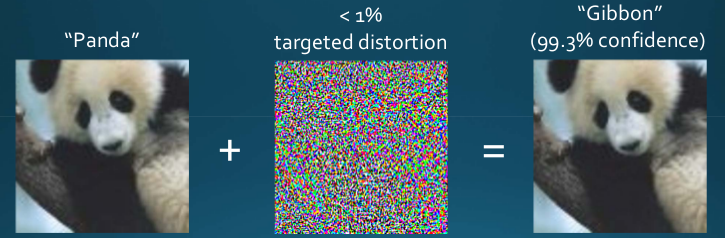
\includegraphics[scale=0.6]{panda-gibbon.png}
  \caption{From \cite{darpa-slides}: Example of the inherent flaws of statistical models: for the human eye, the distorted panda looks almost identical to the original; whereas the trained model predicts a gibbon.}
  \label{fig:panda}
\end{figure}


%% The question wether artificial intelligence is limited to information processing, and/or measured by a combination of those four skills is matter for an interesting discussion, but arguably out of the scope of this thesis. In any case, the points exposed so far enable a way to contextualize and justify the approach taken in this project, namely to use artificial neural networks for music classification:

%% \begin{itemize}
%%         \item As in most art forms, music categories aren't a well-defined problem domain, except for the most trivial cases (and carnatic music is definitely not one of those). So the first-wave approach is discarded: it would be extremely impractical (at best) to attempt to define a rule-based algorithm that describes such complex categories comprehensively.
%%         \item Assuming that no life-critical task would depend on music classification, and that there isn't a systematic to establish that a piece of carnatic music is more relevant than the others, the overall classification success rate is arguably a good measure for the model's success. Following this criteria, statistical models are not excluded.
%%         \item Furthermore, in this project is also assumed that the dataset is comprehensive, correctly labeled, and that carnatic music didn't experience any radical change in the last century. Based on this assumptions, contextual adaptation would be desirable, but not required and third-wave models aren't needed to correctly perform classification on the dataset. It would also follow that the results on the dataset are extrapolable for any kind of current or recorded carnatic music. Of course, this are very strong assumptions and can severely skew the conclusions, but the curation of a dataset or the expertise in the history of carnatic music are matters outside the scope of this thesis.
%%         \item The Dunya dataset is fairly recent, and hasn't been fully explored yet. The range of applications where deep learning models outstand is steadily growing (they conform the state of the art for many classification problems), and the question on how do they perform on that dataset is {\it per se} a legitimate one.
%%         \item Last but not least, there are also practical considerations: statistical models are currently a relevant technology and a sound knowledge on how to design and apply them is not only desirable, but also necessary before critizising and improving them. Context-adaptative approaches are also desirable, but would require sound knowledge in more advanced techniques like covariance propagation, bootstrapping and others that would be more suitable in the context of a more advanced study level.
%% \end{itemize}




\section{Supervised Learning}\label{supervlearning}

As already mentioned, identifying an example as belonging to a category is sometimes much easier as defining the category itself. In that case, the categories can be implicitly defined as a collection of labeled examples, by doing this comprehensively. It is also possible for statistical models to learn categories from a dataset with few or even no labels, by performing unsupervised and semi-supervised learning. But if the dataset has been already labeled (and is assumed to be correct, consistent and comprehensive, as in this thesis), it is more sensible to perform supervised learning, since it profits the most from the extra information provided by each sample's label.\\

This section will describe the general features of every parametric model performing supervised learning, as well as the main strategy to follow: maximizing the likelihood.

\subsection{Setup Formalization}

The task of supervised learning, as described in \cite[Chapter 18]{russell}, is:
\begin{quote}
  Given a \textbf{training set} \((X, y)\) of \(m\) input-output pairs \( (x^{(1)}, y^{(1)}), (x^{(2)}, y^{(2)}), ...  \) \((x^{(m)}, y^{(m)}) \), where each \(y^{(j)}\) was generated by an unknown function \(y = f(x)\), discover a function \(h\) that approximates the {\it true function} \(f\).
\end{quote}
Where each \(x^{(i)}\) is a \textbf{feature vector} in \(\mathbb{R}^n\), having \(n\in\mathbb N_{> 0}\) dimensions (the \textbf{features}) and elements labeled from \(x_1^{(i)}\) to \(x_n^{(i)}\). This specifical kind of dataset is also called labeled, because each \(x^{(i)}\) is coupled to its \textbf{label} \(y^{(i)}\in\(\mathbb{R}\)\). The compact notation \((X, y)\) is used here to refer to the whole dataset, being \(y\in\(\mathbb{R}^m\)\) the vector of labels and \(X\in\mathbb{R}^{m\times n}\) the matrix holding all \(x^{T}\) feature vectors.\\
The defining characteristic of supervised learning is that it is always based on labeled data, and it has two main applications: \textbf{regression}, where \(y^{(i)}\) and the output of \(h\) are real numbers, and \textbf{classification}, where they are discrete. The possible outputs of a classificator are called \textbf{classes}.\\

In this context we define a \textbf{model} where \(h(\theta, x)\) (usually called the \textbf{hypothesis} function) has some \textbf{parameters} or \textbf{weights} \(\theta\) and combines them with the \textbf{input} \(x\) to make its \textbf{prediction}. If there is only a limited set of weights, the model is called \textbf{parametric}. The goal of the training is to adjust those parameters so that \(h\) ends up as close as possible to \(f\). And to get those parameters ``better'' it is needed at first point a criterion to know how ``good'' they are. This is given by the \textbf{cost function} \(J(\theta, X, y)\) (also called \textbf{objective}, \textbf{loss} or \textbf{error} function indistinctly), that performs some kind of comparation between each \(h(\theta, x^{(i)})\) and its respective \(y^{(i)}\), and outputs a non-negative real number representing how bad \(h\) behaves. This number can be interpreted as the ``distance'' between the hypothesis and the true function.


\subsection{Optimization Strategy}

Once we have \(J\) as a way to measure the quality of the parameters, the problem turns into a numerical optimization one, namely:
\begin{equation*}
  \begin{aligned}
    & \theta^* = \underset{\theta}{\text{minimize}}
    & & J(\theta, X, y)
  \end{aligned}
\end{equation*}
Where the best parameters (\(\theta^*\)) are the ones that afford the minimal value of \(J\) for the given dataset. This means \(J\) is used in the model as a criterium not only to \textbf{evaluate} but also to \textbf{learn}.\\

It is important to remark that coming up with a good \(J\) isn't a trivial task: its criterium must be formulated in a concise but general way, but on the other hand it must be kept computationally simple since it must be usually applied many times on big amounts of data. The optimization of \(J\) is also rarely trivial (see \ref{graddesc} for more details and an explanation of the \textbf{gradient descent} algorithm, used in most settings and also in this project for the optimization of \(J\)). For all this reasons, the cost function is one of the most characteristical and important features of a learning model.\\

In this context, and always quoting from \cite[p.131]{goodfellow}: ``Rather than guessing that some function might make a good estimator, we would like to have some principle from which we can derive specific functions that are good estimators for different models. The most common such principle is the \textbf{maximum likelihood principle}.''
``One way to interpret maximum likelihood estimation is to view it as minimizing the dissimilarity between the empirical distribution p̂ data defined by the training set and the model distribution, with the degree of dissimilarity between the two''.

If X represents all our inputs and Y all our observed targets, then the conditional maximum likelihood estimator is:

\begin{equation*}
  \begin{aligned}
    & \theta_{ML} = \underset{\theta}{\text{maximize}}
    & & P(y | X, \theta)
  \end{aligned}
\end{equation*}

And if the examples are assumed to be independent and identically distributed (as we assume for our dataset), then this can be decomposed into:
\begin{equation*}
  \begin{aligned}
    & \theta_{ML} = \underset{\theta}{\text{maximize}}
    & & \sum_{i=1}^m log P(y^{(i)} | x^{(i)}, \theta)
  \end{aligned}
\end{equation*}


Under the right conditions, the main appeal of the maximum likelihood estimator is that it can show \textbf{consistency} (meaning that as the number of training examples approaches infinity, the maximum likelihood estimate of a parameter converges to the true value of the parameter) and \textbf{efficiency} (meaning that compared to other estimators, it will require fewer examples to obtain a fixed level of generalization error). See \cite[p.134]{goodfellow} for a more detailed explanation.


\subsection{Caveats}

The provided explanation so far applies to all the supervised learning techniques explained in the following subsections. Note that it is exposed to many other problems apart from the already mentioned, for instance:
\begin{itemize}
\item It doesn't regard if the modelled \(h\) is complex enough to be able to emulate \(f\), this is something that the designer must care about. On the other hand, if the model is too complex, it may tend to simply memorize the training examples and fail to generalize well, a problem known as \textbf{overfitting}.
\item Even if the model seems adequate, a bad management of the data (for example, testing on the same data that was used to train) or an inconsistent dataset may strongly skew the outcome.
\item Many models are also very sensitive to how the data is formatted, and some simple preprocessing may be recommendable or even necessary (for example, normalizing the data before performing a PCA compression).
\item The total cost or the success ratio aren’t always appropiate ways to measure performance. For example, if some detection problem has only 0.001\% positives, simply assigning every case to negative would provide a 99.999\% accuracy without being useful at all.
\end{itemize}





%%    \section{Linear Regression}\label{linearreg}
%%    This category comprises the regression techniques that base their hypothesis function on a \textbf{dot product} between the input vector \(x\) (passed to some function \(\phi\)) and a parameter vector \(\theta\) of the same dimensionality. It can be thought as ``a sum of elements in the input vector weighted by elements of the parameter vector''\cite[ch. 10.1]{cohen}. In its simplest form, sufficient for this explanation, \(\phi\) is the identity function \(\phi(x)=x\) and can be omitted (alternative strategies for \(\phi\) and their motivations will be discussed in \ref{interaction}). The remaining dot product is a linear function that can be intuitively seen as an ``affinity filter'' between the to-be-learned \(\theta\) vector and the given features, producing its predicted, real-valued output. This is the core idea and that's why it is called linear regression. Actually, what \(h\) performs is an \textbf{affine function}, that is, the explained linear transformation followed by a translation. This translation is necessary to approximate functions with constant components, and is achieved by adding a \textbf{intercept} or \textbf{bias term} \(b\) to the dot product:\\
%%    \begin{equation*}
%%      h(\theta, b, x) = \theta^Tx+b
%%    \end{equation*}

%% Some languages and libraries allow to write this operation directly in this algebraic (so-called \textbf{vectorized} form: for more on vectorization see \ref{vectorization}). Also, for the sake of notation brevity, and as explained in \ref{implicitbias}, this work will use the following {\it implicit bias} notation as equivalent:

%%    \begin{equation*}
%%      h(\theta, x) = \theta^Tx
%%    \end{equation*}


%% \subsection{Hypothesis Function}

%% The simplest case takes place when the input has only one feature (for example, predict the weight of a person based on the height). The hypothesis is in its expanded form \(h(\theta, x)=\theta_0+\theta_1x\), and implies that the model is expected to work well when the {\it true function} behaves close to linearly (example: see figure \ref{fig:unilinreg_b}). In fact, it will reach zero cost if and only if all the points of the dataset are alligned, or ``collinear''.\\

%%  Multivariate linear regression, as the name suggests, applies when the input vector has more than one dimension. For example, predict the prize of a car based on its many features: length, color, horsepower... although an univariate approach based only on the horsepower would probably be effective, taking more features helps to make preciser predictions. It can be intuitively seen as the simultaneous learning of many univariate linear regressions, where all bias terms add up to a single \(\theta_0\), since all of them share the same ``bias feature'' (\(x_0=1\)), and all the other terms are linearly independent from each other. Again, the expanded form of the hypothesis for \(n\) features is: \(h(\theta, x) = \theta_0+\theta_1x_1+\cdots +\theta_nx_n\).


%% \subsection{Cost Function and Optimization Objective}

%%    The linear basis explained so far has the advantage of being stable, and computationally very efficient, especially when combined with the \textbf{mean squared error} (also referred as the \textbf{MSE}, \textbf{L2} or \textbf{euclidean}) cost function: as the name says, it measures the mean of the squared distance between the hypothesis function and the labels. The optimization objective is to minimize it is known as the \textbf{least squares estimation} ({\it LSE}):
%%    \begin{equation*}
%%      \begin{aligned}
%%        & \underset{\theta}{\text{minimize}}
%%        & & J(\theta, X, y) = \frac{1}{2m}\sum_{i=1}^m\{(h(\theta,x^{(i)})-y^{(i)})^2\}
%%      \end{aligned}
%%    \end{equation*}

%% The computational efficiency becomes evident by the fact that the derivative of a square function is a linear function itself. In fact, the \(\frac{1}{2}\) factor is there simply to make the derivative used in the gradient descent equation of \(J\) even more straightforward, as shown below:

%%   \begin{tcolorbox}[ams align*]

%%                The derivative for the mean squared error with respect to a parameter \(\theta_j\) can be calculated following this derivation rules:
%%              \begin{align*}
%%                \begin{aligned}
%%                  &(f(z)+g(z))' = f'(z) + g'(z)\\
%%                  &(f(z)g(z))' = f'(z)g(z) + f(z)g'(z)\\
%%                  &(f(g(z)))' = f'(g(z))\cdot g'(z)\\
%%                \end{aligned}
%%              \end{align*}
%%              Where, in the case of \(J(\theta, X, y) = \frac{1}{2m}\sum_{i=1}^m\{(h(\theta,x^{(i)})-y^{(i)})^2\)\}
%%              \begin{align*}
%%                \begin{aligned}
%%                  & \frac{\partial \frac{1}{2m}}{\partial \theta_j} = 0\\
%%                  & \frac{\partial (\theta^Tx^{(i)}-y^{(i)})^2}{\partial \theta_j} = 2(\theta^Tx^{(i)}-y^{(i)})\cdot x_j^{(i)}\\
%%                \end{aligned}
%%              \end{align*}
%%              Therefore, it holds:
%%              \begin{align*}
%%                \begin{aligned}
%%                  \frac{\partial \(J(\theta, X, y)}{\partial \theta_j} &= \frac{1}{2m} \cdot 2 \{\sum_{i=1}^m(\theta^Tx^{(i)}-y^{(i)})\cdot x_j^{(i)}\}\\
%%                  &= \frac{1}{m} \{\sum_{i=1}^m(\theta^Tx^{(i)}-y^{(i)})\cdot x_j^{(i)}\}\\
%%                \end{aligned}
%%              \end{align*}   % ( \big( \Big( \bigg( \Bigg(
%%               For all \(i\in \{1, ..., m\}\) sample indexes and \(j\in \{1, ..., n+1\}\) dimensions.
%%   \end{tcolorbox}

%% Note that the \(\frac{1}{m}\) normalization factor helps to unify the interpretation of \(J\) and the regularization (see \ref{regularization}) between experiments with different \(m\) (thus it can be ignored if \(m\) is kept constant). With this derivative, the gradient descent equation ends up looking like this (see \ref{graddesc} for more details on gradient descent):




%%    \begin{equation*}
%%      \theta_j := \theta_j-\alpha\frac{\partial J}{\partial\theta_j} = \theta_j-\alpha\frac{1}{m}\sum_{i=1}^m(h(\theta,x^{(i)})-y^{(i)})\cdot x_j^{(i)}
%%    \end{equation*}
%%    Assuming that the data presents independence and linearity among dimensions, or taking the average among the samples as this model does carries some implications that can be problematic, depending on the dataset. In that case, linear regression still has a chance of performing well by using another \(\phi(x)\) that takes interactions and non-linearities into account (see \ref{interaction} for more information on that). For bigger datasets, keeping the computation simple becomes a priority (since it usually helps to overcome those problems too), and a main criterion when choosing a model. In fact, using the {\it LSE} allows to even bypass the whole gradient descent approach, since it yields a convex optimization problem for every possible dataset\cite[p. 719]{russell} (see figure \ref{fig:unilinreg_a} for an example with two parameters), which means that there is a single global optimum that can be calculated analitically (the so-called \textbf{closed-form optimization}. Solving the \textbf{normal equations} for the model achieves exactly that. Since the cost function is quadratic and non-negative, the idea is that the optimized parameters \(\theta^*\) that return the global minimum match the point in which all gradient derivatives equal zero:

%% \begin{tcolorbox}[ams align*]

%% The assumed independence between dimensions allows to formulate the given definition for \(J\) in its vectorized, {\it implicit bias} form:

%% \begin{align*}
%%    \begin{aligned}
%%    J (\theta, X, y) = \frac{1}{2m} (X\theta - y)^T(X\theta - y) \right)
%%    \end{aligned}
%%    \end{align*}

%%    And solving the kernel space of its derivative yields the solution:

%%    \begin{align*}
%%    \begin{aligned}
%%    \frac{\partial}{\partial \theta}  J (\theta^*, X, y) = 0 \iff \frac{\partial}{\partial \theta} \left((X\theta^* - y)^T(X\theta^* - y) \right) = 0\\
%%    \iff \frac{\partial}{\partial \theta} \left(\theta^{*T} X^T X \theta^* - 2\theta^{*T} X^T y+y^T y \right) = 0\\
%%    \implies 2 X^T X \theta^* - 2 X^T y = 0 \\
%%    \implies \theta^* = (X^TX)^{-1}X^T y
%%    \end{aligned}
%%    \end{align*}

%% \end{tcolorbox}



%% See \cite[p. 109]{goodfellow} and (regularization-tikhonov???) for more details on the normal equations. Note that since this method delivers the global optimum in ``one step'', this is usually the preferrable way, unless the number of dimensions \(n\) becomes too big: its computation involves matrix inversion, whose complexity is in $\mathcal{O}(n^3)$ (actually is slightly below), whereas gradient descent is in $\mathcal{O}(n)$\cite{normalequation}. Again, see \ref{graddesc} for the details on gradient descent.\\

%% And last but not least, it can be shown that calculating the {\it LSE} (either with the normal equations of with gradient descent) for the linear regression model yields the same estimate of the \(\theta\)  parameters as does maximizing the log-likelihood\cite[p.134]{goodfellow}, with the corresponding nice properties already mentioned in \ref{supervlearning}.\\

%% For all this reasons, the linear regression + {\it LSE} combo has become the basis for many statistical models, including the most popular and performant ones (like neural networks), so even when linear regression wasn't directly used in the context of this thesis, getting a good intuition on how it works is very recommendable in order to develop and apply those models effectively.



%% \begin{figure}
%%         \centering
%%         \begin{subfigure}[b]{0.4\textwidth}
%%           \centering
%%           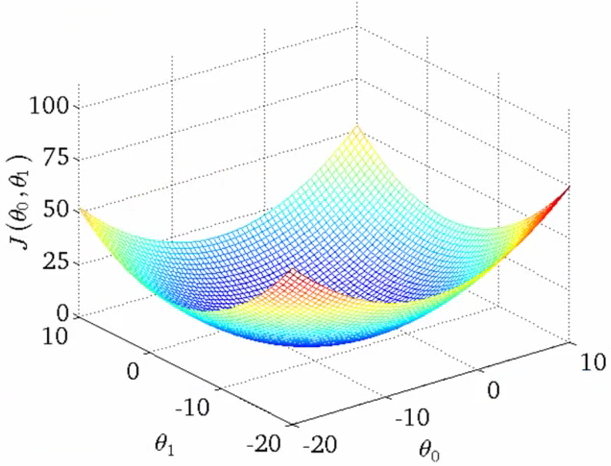
\includegraphics[width=\textwidth]{uni_linreg_j.png}
%%           \caption{An example of \(J(\theta_0, \theta_1)\) from Ng. both moving the th0 and th1 increases quadratically}
%%           \label{fig:unilinreg_a}
%%         \end{subfigure}
%%         \hfill
%%         \begin{subfigure}[b]{0.4\textwidth}
%%           \centering
%%           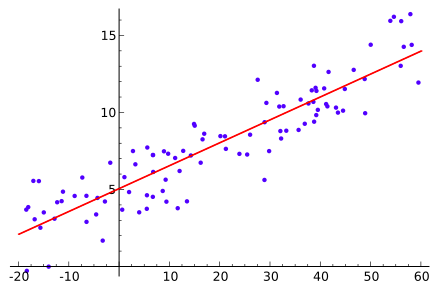
\includegraphics[width=\textwidth]{uni_linreg_h.png}
%%           \caption{an example of \(h(x)\) see how changing th0 (shifting fn) or th1 (gradient) would rise J from wikipedia}
%%           \label{fig:unilinreg_b}
%%         \end{subfigure}
%%         \hfill
%%         \caption{Univariate linear regression: examples for convex \(J\) and optimal \(h\)}
%%         \label{fig:unilinreg}
%%       \end{figure}


\section{Logistic Regression} \label{logreg}

Logistic regression is a classification technique with discrete output. Apart from the fact that classification is required for more complexer tasks, as detection or tracking, logistic regression is especially important in the context of this thesis because it conforms the necessary basis to understand neural networks, as the {\it TensorFlow} API states:
\begin{quote}
  ``The usual method for training a network to perform N-way classification is multinomial logistic regression, aka. softmax regression. Softmax regression applies a softmax nonlinearity to the output of the network and calculates the cross-entropy between the normalized predictions and a 1-hot encoding of the label. For regularization, we also apply the usual weight decay losses to all learned variables. The objective function for the model is the sum of the cross entropy loss and all these weight decay terms, as returned by the loss() function.''\cite{tf-cnn}
\end{quote}

This section will provide a detailed explanation for the multinomial softmax regression, used to classify among \(C\in\mathbb N_{\geq 2}\) different classes, and trained with gradient descent using the cross-entropy as its cost function.

\subsection{Hypothesis for Two-Class Classification}
Any regression model whose hypothesis is based on the \(\theta^T \phi(x)\) dot product can be almost directly used to perform a simple two-class classification: it only needs to be combined with a \textbf{decision boundary}, a real number representing the border between two classes: the positive, labeled as 1 and the negative, labeled with 0. This is achieved by passing the hypothesis to a \textbf{threshold function} (\(Threshold = (\theta^Tx+b)>=t\)), predicting \(x\) as belonging to the \textbf{positive} class when true and \textbf{negative} else, where \(t\in\mathbb{R}\) would be the threshold, usually 0 (again, the identity function \(\phi(x)=x\) is assumed, so it can be omitted until \ref{interaction}). This is the basic idea behind the \textbf{perceptron}\cite[p.729]{russell}, ``the first model that could learn the weights defining the categories given examples of inputs from each category''\cite[p.15]{goodfellow}. A brief and interesting contextualization can be found in the introduction of \cite{vapnik}.\\

But the threshold function has several problems, well summarized in \cite[ch.1]{nielsen} and \cite[p. 725]{russell}: The threshold function is discontinuous, not differentiable and its output announces always a completely confident prediction: 1 or 0. This is problematic for many reasons:
\begin{itemize}
\item Muticlass prediction is not possible: when having more than 2 accepted classes, there is no way to know which one fits best, since all become the same score, a 1.
\item The gradient of the threshold function is always zero except for the boundary, where it is undefined. This makes learning difficult, since it is possible to know if a prediction is false (by comparing it with the label) but not to what extent.
\item Small changes in the hypothesis can produce huge changes in the cost, since all samples that cross the decision border pass from maximal cost to none, or vice versa.
\end{itemize}


\begin{figure}[h]
  \centering
  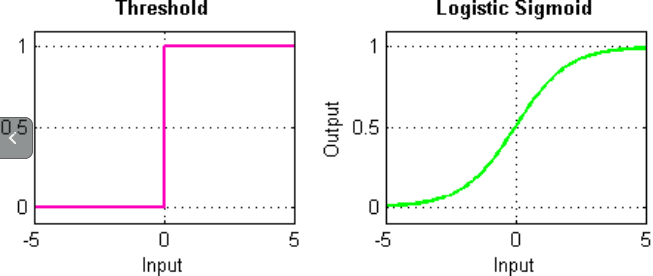
\includegraphics[scale=0.4]{thresh-sig.png}
  \caption{The threshold function with \(t=0\) and the logistic sigmoid\cite{activation-funcs}.}
  \label{fig:sigmoid}
\end{figure}


And there is where logistic regression comes to play: by substituting the threshold function for a softer \textbf{logistic function} (hence the name), all of these issues can be solved to a large extent. For instance, the logistic \textbf{sigmoid} (\(\sigma\)) can be used. It is not as fast to calculate, but it is continuous, differenciable and has a very simple derivative that can be written in terms of its output:

\begin{equation*}
  \sigma(z) = \frac{1}{1+e^{-z}} \qquad \qquad \qquad \frac{d}{dz}\sigma(z) = \sigma(z)(1-\sigma(z))
\end{equation*}\\

This leads to a very efficient calculation, by reusing this output and requiring only one extra subtraction and multiplication. The process of obtaining the derivative will be detailed below.

\begin{tcolorbox}[ams align*]

  The derivative for the sigmoid function can be calculated following the chain rule for derivatives:
  \begin{align*}
    \begin{aligned}
      (f(g(z)))' = f'(g(z))\cdot g'(z)
    \end{aligned}
  \end{align*}
  Where, in the case of \(\sigma(z) = (1+e^{-z})^{-1} = f(g(z))\):
  \begin{align*}
    \begin{aligned}
      & f(z) = z^{-1} \quad \Longrightarrow \quad f'(z) = -z^{-2}\\
      & g(z) = 1+e^{-z} \quad \Longrightarrow \quad g'(z) = -e^{-z}\\
    \end{aligned}
  \end{align*}
  Therefore, it holds:
  \begin{align*}
    \begin{aligned}
      \frac{d}{dz}\sigma(z) = \sigma'(z) &= -(1+e^{-z})^{-2} \cdot -(e^{-z})\\
      & = \frac{e^{-z}}{(1+e^{-z})^{2}}\\
      & = \frac{1}{1+e^{-z}} \cdot \frac{e^{-z}}{1+e^{-z}}\\
      & = \sigma(z) \cdot \frac{1+e^{-z}-1}{1+e^{-z}}\\
      & = \sigma(z) \cdot  \big( \frac{1+e^{-z}}{1+ e^{-z}} - \frac{1}{1+e^{-z}} \big)\\
      & = \sigma(z) \cdot (1 - \sigma(z))\\
    \end{aligned}
  \end{align*}   % ( \big( \Big( \bigg( \Bigg(
\end{tcolorbox}

In the context of neural networks, such functions as the threshold and the sigmoid are called \textbf{activation functions}, because of the analogy to neurons (more on this in section \ref{neuralnetworks}). For a visual comparation between some different activation functions see Figure \ref{fig:sigmoid} .\\


The sigmoid also allows a more refined interpretation: its output can be seen as a probability distribution \(P(y=1|x)\)\cite[p.181]{goodfellow} continuous in the \((0, 1)\) range, and the decision boundary can now be obtained by choosing any \(t\) in such range. The standard is \(t=0.5\), since the probability distribution can be now interpreted as the ``degree of belief'' the system has, being results close to 1 clear positives and results close to 0 clear negatives (note that \(\sigma(z)=0.5\) means that \(z=0\), see \ref{errormetrics} for more information about choosing different values for \(t\)). In this context, the \(z = \theta^Tx\) variable ``defining such a distribution over binary variables is called a \textbf{logit}''\cite[p.182]{goodfellow}.\\

Now it is possible to define the hypothesis for the two-class logistic regression with sigmoid activation function, by \(z\) with \(\theta^Tx\) as the sigmoid's argument:

\begin{equation*}
  h(\theta, x) = \sigma(\theta^Tx) \qquad \qquad \qquad x \text{ is positive} \iff h(\theta, x)>=t\\
\end{equation*}

And last but not least, this hypothesis, combined with the proper cost function, leads to a very efficient formula for the gradient descent algorithm that maximizes the likelihood\cite[p.184]{goodfellow}, with the corresponding nice properties already mentioned in \ref{supervlearning}. This will be explained in detail after describing the multinomial version of the logistic regression, which is a generalization of the two-class model explained so far and shares the same gradient descent formula and likelihood maximization properties.


%% The nice properties of this function apply also when its gradient is used in order to {\it learn} those parameters (see \ref{graddesc} for more details on gradient descent): not only the gradient can be efficiently calculated as already explained, but also it is very adequate: its steepness is maximal in the middle and converges to zero in both extremes. The intuition behind that is that if the sigmoid is interpreted as the ``degree of belief'', the steepness can be seen as the ``permeability to different beliefs'', following the analogy: The more certain the prediction is, the less prone to change will it be. So if gradient descent is initialized in a way that every prediction starts close to the ``center'' (which represents the total uncertainty), the parameters will be able to keep maneuvrability until the predictions converge to one side or the other.\\

%% In this context, the naive approach for a cost function \(J\) would be simply to take the mean square error between each label and the corresponding prediction, as with logistic regression, and then minimize it with gradient descent [QUESTION: IS IT FEASIBLE TO SOLVE IN CLOSED-FORM WITH SIGMOID+MSE?]. This would actually be very problematic, since it would make almost impossible to correct big errors using gradient descent: the gradient of \(J\) for such cases (that is, when \(h\) predicts a value close to 0 but 1 was expected, or vice versa) would be almost zero (see \cite{softmax}), and the model should be able to learn from every failure, especially the big ones.\\

%% So the challenge here is to find a function that avoids this problem, but keeping at the same time the nice properties of the sigmoid: that is exactly what the \textbf{cross-entropy} achieves. But due to the fact that the approach explained so far for two classes is the simplest form of a more general model with \(C\in\mathbb{N}_{\geq2}\) classes, this will be explained in the next subsections in order to avoid duplicity.

\subsection{Hypothesis for Multinomial Classification} \label{multiclass}
Multinomial classification answers the question: ``Having \(C\in\mathbb{N}_{\geq2}\) classes, Which class \(c\in C\) does \(x\) belong to?''. To answer this, it suffices to apply the sigmoid model seen so far multiple times, with a different set of parameters for each class, and picking the answer with the biggest output. But when classifying between disjoint classes (which means the samples can only belong to one class), raising one outcome should obviously reduce the others. The multiple sigmoid approach deprives the model of this knowledge, which is not optimal\cite{softmax}. The \textbf{softmax function} adresses this issue. It ``can be seen as a generalization of the sigmoid function''\cite[p.183]{goodfellow}, and is ``a way of forcing the outputs of \(h\) to sum to 1, so that they can represent the probability distribution across discrete, mutually exclusive alternatives''\cite{softmax}:

\begin{equation*}
  S(z)_c = \frac{e^{z_c}}{\sum_{j=1}^C(e^{z_j})}\\[3mm]
\end{equation*}

In this case, instead of a scalar, this function accepts a \(z\in \mathbb{R}^C\) logit vector and returns a vector of same dimensionality. This output vector behaves also as a probability distribution \(P(y=c | x)\), holding the ``degree of belief'' for each \(z_i\) logit: every output is in the range \((0, 1)\), and the sum of all its outputs is always 1. And, analogous to the sigmoid, its derivative can be also expressed in terms of its output, but the derivation is a little more involved, since it requires some notions on vector calculus. Specifically, the dimension of both output and input components has to be specified:
\begin{equation*}
  \frac{\partial S(z)_a}{\partial z_b} \qquad a,b \in \{1, ..., C\}\\[3mm] %  = S(z)_c(1-S(z)_c)
\end{equation*}

Thus, the complete definition of the derivative comprises \(C\times C\) partial derivatives, which are usually displayed in a matrix called the \textbf{jacobian}\cite[p.86]{goodfellow}. The derivative is explained below.\\

As a side note regarding the properties of the softmax function, dividing the logit vector by a scalar \(\mu\in\mathbb{R}_{>1}\) before passing it to \(S\) will tend to uniformize the output distribution, and multiplying to polarize its belief towards the output with the maximal score. This property can be used to regulate the ``radicality'' of the classificator, which could tend to either equalize or magnify the actual differences. Also, as usual in exponential functions, there are some numerical issues that must have be taken into account, to avoid over- and underflowing when performing their calculation. This is worth to mention, but the present project relies on lower-level libraries to provide a stable implementation and therefore won't be further covered (see \cite[p.81 and p.185]{goodfellow} for more details).


\begin{tcolorbox}[ams align*]

  The jacobian for the softmax function can be calculated following the derivation rule for division:

  \begin{align*}
    \begin{aligned}
      \Big( \frac{f(z)}{g(z)}\Big)' = \frac{f'(z)g(z) - f(z)g'(z)}{g(z)^2}
    \end{aligned}
  \end{align*}
  Where, in the case of \(S(z)_a = \frac{f(z)_a}{g(z)}\):
  \begin{align*}
    \begin{aligned}
      & f(z)_a = e^{z_a} \quad \Longrightarrow \quad \frac{\partial f(z)_a}{\partial z_b}
      = \begin{dcases}
        e^{z_a} = e^{z_b} & \text{if } a=b\\
        0     & \text{otherwise}
      \end{dcases}\\
      & g(z) = \sum_{j=1}^C(e^{z_j}) \quad \Longrightarrow \frac{\partial g(z)}{\partial z_b} = e^{z_b}\\
    \end{aligned}
  \end{align*}
  Therefore, it holds:
  \begin{align*}
    \begin{aligned}
      \frac{\partial S(z)_a}{\partial z_b} = \begin{dcases}
        \frac{e^{z_a}g(z)-e^{z_a}e^{z_b}}{g(z)^2} = \frac{e^{z_a}(g(z)-e^{z_b})}{g(z)g(z)}  = S(z)_a(1-S(z)_a)       & \text{if } a=b\\
        \frac{0g(z)-e^{z_a}e^{z_b}}{g(z)g(z)} = -\frac{e^{z_a}}{g(z)}\frac{e^{z_b}}{g(z)} = -S(z)_a S(z)_b
        & \text{otherwise}
      \end{dcases}\\
    \end{aligned}
  \end{align*}   % ( \big( \Big( \bigg( \Bigg(
  Or, abbreviated:
  \begin{align*}
    \begin{aligned}
      \frac{\partial S(z)_a}{\partial z_b} = S(z)_a(\mathbbm{1}_{i=j}-S(z)_b)
    \end{aligned}
  \end{align*}   % ( \big( \Big( \bigg( \Bigg(
  Where \(a,b\) would also denote the corresponding index in the jacobian matrix.
\end{tcolorbox}


Having this explained, the hypothesis the multinomial version of \(h\) can be now formulated by substituting each \(z_c^{(i)}\) in the softmax function with the actual logit \(\theta_c^Tx^{(i)}\). That means, the model needs \textbf{one \(\theta_c\) parameter vector per class}. In this context, \(h\) can be more generally formulated as follows:\\
\begin{equation*}
  h(\Theta, x)_c = S(\Theta^Tx)_c \qquad \qquad \qquad class(x) = index(max(h(\Theta, x)))\\[3mm]
\end{equation*}
Where \(x\) is still the same feature vector in \(\mathbb{R}^{(n+1)}\) (holding \(n\) features {\it plus the implicit bias}, see \ref{implicitbias}), and \(\Theta\in\mathbb{R}^{(n+1)\times C}\) is a matrix that holds all parameter vectors (one for each class), so the output of \(h\) (as well as the bias term \(b\)) is now a vector with \(C\) dimensions (holding one prediction per class).\\

Especially, note that {\it the one-dimensional version of softmax and its derivative are equal to the two-class model using the sigmoid}. This makes easier to see why this model is a generalization of the former, but there is one notational inconsistency: for \(C\) classes softmax accepts a vector with \(C\) dimensions, whereas for two classes the sigmoid accepts a single scalar instead of a two-dimensional vector.\\

And not only that: a naive implementation of a two-class problem using the general model implementation would require a \((2\times C)\) matrix instead of a \(C\)-dimensional vector, with the corresponding memory and computational overhead. This is worth to note, and should be handled properly when implementing the low-level algorithms, but won't be covered here. Instead, and for convenience reasons, the general notation will be used here for any classification problem with \(C\in \mathbb{N}_{\geq 2}\).\\

It only remains one more inconsistency before finally tackling the cost function and optimization objective for the multinomial logistic regression: the output of the hypothesis for the \(x^{(i)}\) sample is a vector, whereas the predicted label \(class(x^{(i)})\) is a scalar. In this form, a direct comparation between hypothesis and labels is undefined. This is solved by adapting the labels to the so-called \textbf{one-hot} format, explained in the next section.

\subsection{One-Hot Encoding}

As explained before, the output of the hypothesis is a discrete probability distribution in \((0,1)^C\), but the \(y^{(i)}\) labels in the training set are natural numbers in \(\{1, ..., C\}\). In its \textbf{one-hot} version, the natural number \(y^{(i)} = c\in C\) corresponding to the labeled class is converted to a \(\vec{y}\) vector with \(C\) dimensions where all \(\vec{y_i}\) entries are 0 except \(\vec{y_c}\), which is 1:
\begin{equation*}
  y^{(i)}= c  \iff \vec{y}= \begin{bmatrix}y_0 = 0 \\ y_1 = 0 \\ \vdots \\ y_c = 1 \\ \vdots \\ y_C = 0\end{bmatrix}
\end{equation*}
This vector can be now formally compared with the output of \(h\). Note that there are no negative classes in this context, since every one-hot encoded label is positive to exactly one class (a two-class classification would have this way a two-dimensional vector instead of a boolean scalar).



\subsection{Cost Function and Optimization Objective}\label{logregcost}

The cost function used to measure the difference between the hypothesis and the dataset labels is called \textbf{cross-entropy}, designated here with the letter \(\mathcal{L}\) (see \ref{kldivergence} for a more detailed background):

\begin{equation*}
  \mathcal{L}(P, Q) = -\sum_{i=1}^{m} \Big\{P(\epsilon_{ic}) log(Q(\epsilon_{ic})) \Big\}\\[3mm]
\end{equation*}

Whereas the event \(\epsilon_{ic} := \{Y_i=c\}\) corresponds to the \(i^{th}\) sample of some random variable \(Y\) belonging to class \(c\). As we assume that the samples in the dataset are independent and identically distributed (i.i.d), the formula translated to the model explained so far (including the one-hot encoded \(\vec{y}\) labels) turns into:

\begin{equation*}
  J(\Theta, X, y) = -\frac{1}{m}\sum_{i=1}^m \Big\{ log \big(S(\Theta^Tx^{(i)})^T \cdot \vec{y}^{\:(i)} \big) \Big\}\\[3mm]
\end{equation*}


As already anticipated, the optimization of this cost function is equivalent to maximizing the likelihood (with the corresponding consistency and efficiency properties already mentioned in \ref{supervlearning}). Quoting from  \cite[p.184]{goodfellow}:

\begin{quote}
  ``As with the logistic sigmoid, the use of the exp function works very well when training the softmax to output a target value y using maximum log-likelihood [...]. Defining the softmax in terms of exp is natural because the log in the log-likelihood can undo the exp of the softmax''.
\end{quote}


And also importantly, it is very convenient for the optimization with the gradient descent algorithm since its derivative is very efficient to calculate. For instance, note that due to the one-hot encoding, only the \(\vec{y}^{\:(i)}_c = 1\)  component of the label contributes to the dot product with \(S\) (and hence to the cost), so the rest of the components don't have to be calculated. Also, in a {\it i.i.d.} discrete distribution, every sample has a \(P(x^{(i)}) = \frac{1}{m}\), so the term is the same for all of them and can be taken out of the summation. And last but not least, the fact that ``\textbf{the steepness of \(\mathcal{L}\) exactly balances the flatness of \(S\)}''\cite{softmax} allows a great simplification of the derivative, which ends up looking like this (see below for a detailed explanation):

\begin{equation*}
  \frac{\partial}{\partial \Theta}J(\Theta, X, y) = \frac{1}{m}\sum_{i=1}^m \Big\{ (S(\Theta^T x^{\:(i)}) - \vec{y}^{\:(i)}) \cdot x^{\:(i)}^T \Big\} \in \mathbb{R}^{C \times (n+1)}\\[-5mm]
\end{equation*}

This way, the update equation for the gradient descent remains as follows (more information about gradient descent in \ref{graddesc}):


\begin{equation*}
  \begin{aligned}
    \Theta_{next} :&=  \Theta_{current} - \alpha \frac{\partial}{\partial\Theta}J(\Theta_{current}, X, y) \\[3mm]
    &= \Theta_{current} - \frac{\alpha}{m}\sum_{i=1}^m \Big\{ (S(\Theta_{current}^T x^{\:(i)}) - \vec{y}^{\:(i)}) \cdot x^{\:(i)}^T \Big\}\\[3mm]
  \end{aligned}
\end{equation*}

As a side remark, note its great similarity with the gradient descent formula for linear regression.



%% This allows the following reformulation:

%%  \begin{equation*}
%%        J(\Theta, X, y) = -\frac{1}{m}\sum_{i=1}^m \Big\{ log \big(S(\Theta^Tx^{(i)})_{yi}\big) \Big\}\\[3mm]
%%      \end{equation*}

%% With \(S(z)_{yi}\) being the component of the softmax output indexed by the \(y^{(i)} \in \{1, ..., C\}\) label.\\




%% \begin{equation*}
%%      &\frac{\partial}{\partial \Theta_{a,b}} J(\Theta, x^{(i)}, \vec{y}^{\;(i)})  = \begin{dcases}
%%                                     (S(\Theta^Tx^{(i)})-\vec{y}^{\:(i)})x_b^{\:(i)} & \text{if } a=yi\\
%%                                     0  & \text{otherwise}
%%                                     \end{dcases}\\[0mm]
%%      \end{equation*}




\begin{tcolorbox}[ams align*]

  The derivative for the cross-entropy function of the softmax logistic regression (see \cite{softmax} for more references)\\[-20]

  \begin{equation*}
    J(\Theta, X, y) = -\frac{1}{m}\sum_{i=1}^m \Big\{ log \big(S(\Theta^Tx^{(i)})^T \cdot \vec{y}^{\:(i)} \big) \Big\}
  \end{equation*}

  with respect to a parameter \(\Theta_{a,b} \in \mathbb{R}\) (corresponding to class \(a \in \{1, ..., C\}\) and dimension \(b \in \{1, ..., n+1\}\)) can be calculated by applying the multivariate chain rule for multiple nested functions, that is, multiplication of jacobian matrices. But this would yield a very sparse matrix (many entries as it is shown, would be zero), so it can be much more efficiently calculated by treating the functions as univariate derivatives for different cases:

  \begin{equation*}
    % \frac{\partial J}{\partial \Theta_{a,b}} = \frac{\partial J}{\partial S_a}\frac{\partial S_a}{\partial h_a}\frac{\partial h_a}{\partial \Theta_{a,b}}\\[3mm]
    \frac{\partial f(g(h))}{\partial \Theta_{a,b}} = \frac{\partial f}{\partial g} \cdot \frac{\partial g}{\partial h} \cdot \frac{\partial h}{\partial \Theta_{a,b}}\\[1mm]
  \end{equation*}

  This way, the function composition \(f(g(h)) = -log(S(\Theta^Tx^{\:(i)})^T \cdot \vec{y}^{\:(i)})\) represents the cost for the \(i^{th}\) sample, having the following components:
  \begin{align*}
    \begin{aligned}
      &h = \Theta^Tx^{\:(i)} \in \mathbb{R}^C := \text{logit for sample } x^{\:(i)} \in \mathbb{R}^{n+1}\\
      &g = S(z)^T \vec{y}^{\:(i)} = S(z)_c \in (0, 1) := \text{labeled component of the softmax function}\\
      &f= -log(\epsilon) := \text{{\it self-information} of the probability of an event } \epsilon \in [0,1]\\[1mm]
    \end{aligned}
  \end{align*}
  In this context, the partial derivatives of those components are the following:
  \begin{align*}
    \begin{aligned}
      &\frac{\partial h}{\partial \Theta_{a,b}} = \frac{\partial (\Theta^Tx^{\:(i)})}{\partial \Theta_{a,b}}
      % = \frac{\partial (\Theta_{(a,\, ...)}x^{\:(i)})}{\partial \Theta_{a,b}}
      = x^{\:(i)}_b\ \quad \text{(the \(x_{v \neq b}\) components don't interfere)}\\
      &\frac{\partial g}{\partial h} = \frac{\partial S(h)_c}{\partial h} = \begin{dcases}
        S(h)_{c}(1-S(h)_{c}) & \text{if } a=c\\
        S(h)_{c}(0-S(h)_{c})  & \text{otherwise}
      \end{dcases}\\
      &\frac{\partial f}{\partial g}= \frac{\partial(-log(S))}{\partial S} := -\frac{1}{S}\\[-0mm]
    \end{aligned}
  \end{align*}

  See \ref{multiclass} for a detailed derivation of the softmax function. Now it is possible to apply the chain rule to obtain the derivative of the cost for the \(i^{th}\) sample whit respect to the parameter \(\Theta_{a,b}\):\\[-10mm]

  \begin{equation*}
    &\frac{\partial f(g(h))}{\partial \Theta_{a,b}} = \begin{dcases}
      -\frac{1}{S(h)_c} \; S(h)_c(1-S(h)_c) \; x_b^{\:(i)} = (S(h)_c-1)x_b^{\:(i)} & \text{if } a=c\\
      -\frac{1}{S(h)_c} \; S(h)_c(0-S(h)_c) \; x_b^{\:(i)} = (S(h)_c-0)x_b^{\:(i)}  & \text{otherwise}
    \end{dcases}\\[0mm]
  \end{equation*}

  Which very nicely allows to express all the derivatives for the \(\Theta\) matrix at once by using the one-hot encoded label:
  \begin{equation*}
    &\frac{\partial f(g(h))}{\partial \Theta} = \Big( (S(\Theta^T x^{\:(i)}) - \vec{y}^{\:(i)}) \cdot x^{\:(i)}^T \Big) \in \mathbb{R}^{C \times (n+1)}\\[-2mm]
  \end{equation*}
  The derivative for \(J\) over the whole dataset would be then the mean of this derivative for all \(m\) samples.\\[-13mm]
\end{tcolorbox}



\subsection{Final Intuition on Logistic Regression}

Summarizing, logistic regression is a classifying method whose hypothesis function is an affine function that is passed to a logistic layer. The logistic layer allows it to output a degree of confidence for every class, and to learn efficiently from that information.\\

In order to learn, the cross-entropy with softmax can be conveniently used as cost function: not only it is very effective and fast to calculate, but it also ends up being very intuitive: \textbf{the size of the gradient is directly proportional to the size of the error}, which makes it a very natural criterion to correct the difference between labels and hypothesis. This can be clearly seen in the update formula for the gradient descent algorithm.\\

This way, by starting with a very low confidence everywhere (usually \(\Theta\) as a zero matrix, which should cause a numerically stable softmax to output an uniform distribution), the optimization of \(J\) becomes a ``confidence raising process'', in which each labeled example forces the parameters to get away from zero, in order to approximate the response of \(h\) to the corresponding one-hot label: the prediction for the labeled class should get closer to 1, and the rest of predictions to 0. With this process, the model ends up capturing the features that the classes in the dataset may have, since it performs a maximum likelihood estimation. Nevertheless, logistic regression is a linear model and therefore it has its limitations, as it will be discussed in the next section.\\


\section{Non-Linear Hypothesis}\label{interaction}

The linear basis for the logistic regression explained so far, based on the dot product \(\theta^T\phi(x)\), assumes the use of the identity function \(\phi(x)=x\), which results in a linear hypothesis. In that case, the solution provided by the model is a linear combination of linear functions (in the case of the classificators, the boundary of a linear problem is a {\it hyperplane}).  This can be a valid solution for many problems, but many others won't fit into that assumption. For instance, Minsky and Papert demonstrated in 1969 that the linear perceptron cannot solve functions like XOR or NXOR (as explained and exemplified in \cite[p. 10]{deephist}). Moreover, such linear models ``cannot understand the interaction between any two input variables''\cite[p. 169]{goodfellow}.\\

Actually, for many problem domains it is safe to assume that such interactions and non-linear behaviours are present, and, if that is the case, the ability to craft a non-linear hypothesis can lead to a better solution and is desirable. This is done by using a different \(\phi\) function. As explained in \cite[p.169]{goodfellow}, there are three main strategies:
\begin{enumerate}
\item Handcraft \(\phi\). This was the dominant approach until the advent of deep learning. It can be very effective and efficient, but requires high specialization and has little transfer between domains.
\item Choose a very generic \(\phi\) that maps the data to a very high-dimensional space, and work linearly on that space. If the dimensionality is high enough, we can always have enough capacity to fit the training set, but generalization to the test set often remains poor.
\item Let the model itself learn \(\phi\) (the approach of neural networks). This enables the model to capture the benefits of the other approaches, with the drawback that it is the only variant that gives up the convexity.
\end{enumerate}

The implications and details of this approaches will be briefly discussed in the next subsections.


\subsection{Handcrafted Mapping}

By handcrafting the \(\phi(x)\) function to be a polynomial (or equivalent) function it is possible for the hypothesis to capture specific non-linearities and the so-called \textbf{interaction features} without giving up the linearity of the model: it still behaves as a multivariate linear regression, since it is linear respect to the \(\theta\) parameters, and therefore the optimization of \(J\) still works the same as in the linear models explained so far. The following examples help to illustrate how this works:

\begin{itemize}
\item It may be observed that the rent prices in some city grow quadratically when approaching the center. In that case, a polynomial of degree 2 would make appropiate predictions: \(h(\theta, x) = \theta_0+\theta_1x_1+\theta_2x_1^2\). Here, \(h\) has 3 parameters, although the original data has only a single feature (\(x_1\)), representing the distance to the city center.
\item Two different parameters may also interact with each other, like predicting the prize of a car insurance given age (\(x_1\)) and vision capacity (\(x_2\)): the following hypothesis is able to represent even elliptic and hyperbolic curves: \(h(\theta, x) = \theta_0+\theta_1x_1+\theta_2x_2+\theta_3x_1x_2+\theta_4x_1^2+\theta_5x_2^2\).
\end{itemize}

The intuition behind this examples is the following:  both \textbf{embed} the data into a higher dimensional space, in which they find a linear hypothesis that will reflect the ground truth more closely, or, at least, perform as good as a linear hypothesis (by optimizing the non-linear \(\theta\) coefficients to zero). In fact:
\begin{quote}
  ``\textbf{If the data samples are mapped into a space of sufficiently high dimension, then they will be almost always linearly separable} ---if you look at a set of points from enough directions, you'll find a way to make them line up [...] four dimensions suffice for linearly separating a circle anywhere in the plane (not just at the origin), and five dimensions suffice to linearly separate any ellipse. In general (with some special cases excepted) if we have \(N\) data points then they will always be separable in spaces of \(N-1\) dimensions or more''\cite[p. 746]{russell}.
\end{quote}

\begin{figure}
  \centering
  \begin{subfigure}[b]{0.36\textwidth}
    \centering
    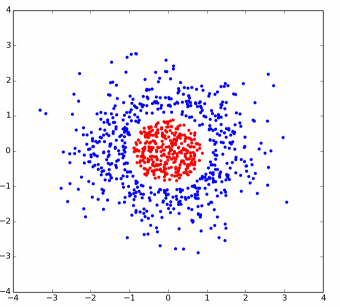
\includegraphics[width=\textwidth]{interact-ft1.png}
    \caption{original 2D dataset}
    %\label{}
  \end{subfigure}
  \hfill
  \begin{subfigure}[b]{0.5\textwidth}
    \centering
    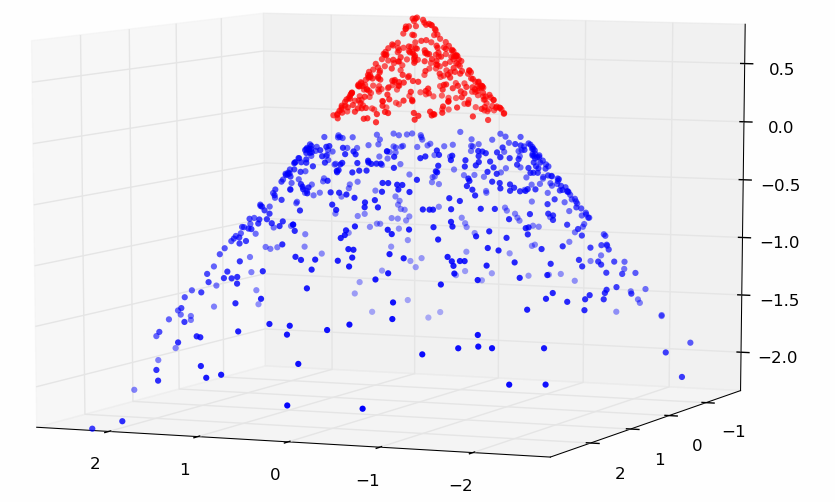
\includegraphics[width=\textwidth]{interact-ft2.png}
    \caption{dataset embedded to a 3^{rd} dimension\\\(\;z = 1-\sqrt{x^2 + y^2}\) becomes linearly separable at \(z=0\)}
    %\label{}
  \end{subfigure}
  \hfill
  \caption{http://stackoverflow.com/questions/1148513/difference-between-a-linear-problem-and-a-non-linear-problem-essence-of-dot-pro}
  \label{fig:interact}
\end{figure}

See figure \ref{fig:interact} to complete this intuition with an example of a classification problem. As a side remark regarding the use of a polynomial \(\phi\), note that it can be desirable to apply mean normalization when optimizing with gradient descent, since the ranges of the features grow very fast when multiplied/exponentiated, and this can delay or even skew the convergence of the algorithm. Actually, and depending on the used software, even optimizing with the normal equations may also benefit from to normalizing the data to avoid error propagation (see {\it poor conditioning}, \cite[p.82]{goodfellow} for more information).\\


\subsection{Generic Mapping}

Ideally, \(\phi\) is handcrafted to provide the smallest embedding possible to effectively model the data. But note that the number of parameter combinations grows exponentially with the number of dimensions, so choosing by hand which combination fits best can become a very time-consuming and is reasonable only in a small scale.Rather,  the \textbf{kernel trick} can be used. Quoting \cite[p.141]{goodfellow}, it ``consists of observing that many machine learning algorithms can be written exclusively in terms of dot products between examples''. For instance, it can be shown that

\begin{equation*}
  \begin{aligned}
    \theta^T\phi(x) = \sum_i^m \{ \alpha_i \phi(x)^T\phi(x^{(i)})\}
  \end{aligned}
\end{equation*}

Where \(x\) is the current input, \((x^{(1)}, ..., x^{(m)})\) the training examples and \(\alpha\) a vector of coefficients. Quoting further,
\begin{quote}
  ``Rewriting the learning algorithm this way allows us to replace x by the output of a given feature function \(\phi(x)\) and the dot product with a function \(k(x, x^{(i)}) = \phi(x)^T\phi(x^{(i)})\) called a kernel [...]. The kernel trick is powerful for two reasons. First, it allows us to learn models that are nonlinear as a function of x using convex optimization techniques that are guaranteed to converge efficiently. This is possible because the optimization algorithm can view the decision function as being linear in a different space. Second, the kernel function k often admits an implementation that is significantly more computational efficient than naively constructing two \(\phi(x)\) vectors and explicitly taking their dot product.In some cases, it can even be infinite dimensional (using, for example, the \textbf{RBF} kernel function), which would result in an infinite computational cost for the naive, explicit approach [...]. The category of algorithms that employ the kernel trick is known as \textbf{kernel machines} or \textbf{kernel methods}''.\cite[p.141]{goodfellow}
\end{quote}

Because of this nice properties, kernel machines, like like the {\it Support Vector Machines}, are a very reasonable off-the-shelf model for many problem domains. But they also present disadvantages. One of them, already anticipated, is that they often lack generalization ability. Also, they don't scalate well for big datasets: the evaluation of the hypothesis function is linear to the number of samples, and:

\begin{quote}
  ``Prior to the advent of deep learning, the main way to learn nonlinear models was to use the kernel trick in combination with a linear model. Many kernel learning algorithms require constructing an \(m\times m\) matrix \(G_{i,j} = k(x^{(i)},x^{(j)})\). Constructing this matrix has computational cost $\mathcal{O}(n^2)$, which is clearly undesirable for big datasets. In academia, starting in 2006, deep learning was initially interesting because it was able to generalize to new examples better than competing algorithms when trained on medium-sized datasets with tens of thousands of examples. Soon after, deep learning garnered additional interest in industry, because it provided a scalable way of training nonlinear models on large datasets.''\cite[p.152]{goodfellow}
\end{quote}

For this reasons, kernel machines weren't used in the context of this thesis and therefore won't be further covered.


\section{Neural Networks}\label{neuralnetworks}

Neural networks can be thought as a stack of linear classifiers on the top of each other, interleaved with some activation layer to avoid the so-called {\it linear lasagna} (since a linear combination of linear layers is equivalent to a single linear layer).\\

See Figure \ref{fig:neurons} for an illustration of the natural and artificial models for a neuron. This basic concept allows a great flexibility: the approaches explained so far have an explicit separation between designing the model and training it on the data. This is the main difference with neural networks: instead of directly mapping the data to a certain space, this models perform multiple mappings, which are learned during the training: the initial one becomes the data, and the last one outputs the classification; but the intermediate ones are learned by the model.\\

This can be put under the broad category of \textbf{representation learning}: ``the last layer of the network is typically a linear classifier, such as a softmax regression classifier. The rest of the network learns to provide a representation to this classifier. Training with a supervised criterion naturally leads to the representation at every hidden layer (but more so near the top hidden layer) taking on properties that make the classification task easier. For example, classes that were not linearly separable in the input features may become linearly separable in the last hidden layer''\cite[p.530]{goodfellow}. There are many ways to implement this idea. In fact, the great flexibility that NN-related models show is one of their strengths, since it makes easier to compromise between hand-engineeried parts and end-to-end training.\\

But this flexibility has also a drawback: the more abstraction is managed by the model, the harder can become for us to interpret what is happening and why is working. This empirical approach is known as \textbf{end-to-end}, because the setup only has explicit control over both the input and the output.\\

The main way of classifying neural networks is by the linear operation that they perform in their layers. If the operation is a matrix-multiplication, that layer is said to be a fully conected, because the matrix contains a weight for every single row-to-column pair, representing the connections between every column-neuron to every row-neuron. The other main type of linear operation, relevant for this thesis, is the convolution. As explained in \cite[p.176]{goodfellow} ``Designing and training a neural network is not much different from training any other machine learning model with gradient descent''. In fact, the only main difference and one of the main reasons of the success of neural networks is the application of the \textbf{backpropagation} algorithm, which leverages the application of the chain rule for specific families of functions in order to compute the derivatives across the layers of the neural network very efficiently. See \cite[p.203]{goodfellow} for a detailled explanation on backpropagation for the different families of neural networks.\\

Another important factor involving the definition of a neural network is the activation function used. ``In modern neural networks, the default recommendation is to use the ReLU''\cite[p.173]{goodfellow}. ReLU is an acronym for Rectified Linear Unit, which in its basic form is the function \(f(x) = max(0, x)\). Its simplicity gets reflected in the numerical stability and computational simplicity of its derivative, which makes it very suitable for ``modern'' networks, which usually feature more layers and representational power. The other prominent activation function, the sigmoid/softmax family, has already been explained in section \ref{logreg}.\\

\begin{figure}
  \centering
  \begin{subfigure}[b]{0.35\textwidth}
    \centering
    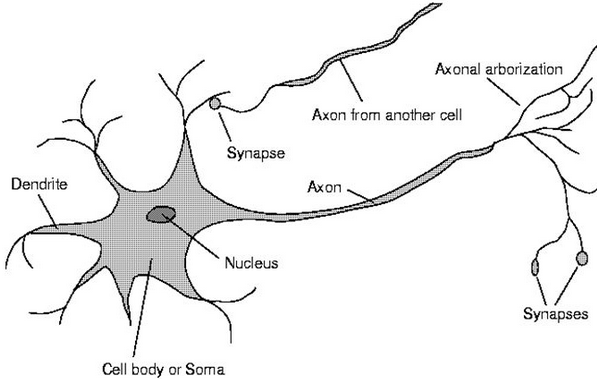
\includegraphics[width=\textwidth]{neuron.png}
    \caption{``The parts of a nerve cell or neuron'', from \cite[p.11]{russell}}
    \label{fig:neuron}
  \end{subfigure}
  \hfill
  \begin{subfigure}[b]{0.6\textwidth}
    \centering
    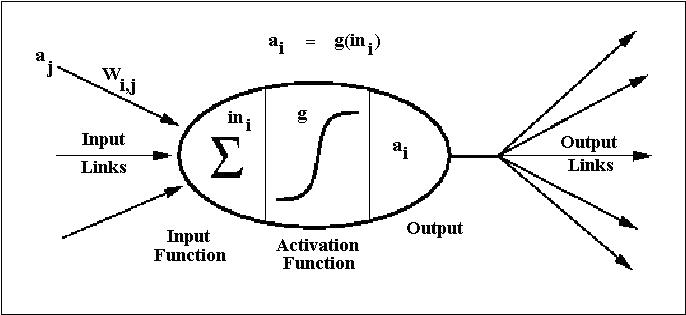
\includegraphics[width=\textwidth]{neuron-model.png}
    \caption{``A simple mathematical model for a neuron'', from \cite[p.728]{russell}}
    \label{fig:neuron-model}
  \end{subfigure}
  \hfill
  \caption{``One should not view deep learning as an attempt to simulate the brain [...]: it is primarily concerned with how to build computer systems that are able to successfully solve tasks requiring intelligence, while the field of computational neuroscience is primarily concerned with building more accurate models of how the brain actually works.''\cite[p.17]{goodfellow}}
  \label{fig:neurons}
\end{figure}


\subsection{Convolutional Networks}

\subsubsection{Parameter Sharing}

Fully connected layers have a great representational power, but it has been shown that deeper networks with smaller layers are more meaningful and perform empirically better\cite[p.202]{goodfellow}. One key concept in this context is the idea of parameter sharing, ``a way to express our prior knowledge about suitable values of the model parameters, by, for instance, forcing sets of parameters to be equal''\cite[p.251]{goodfellow}. This has been proven especially helpful with convolutional networks, which naturally capture such prior knowledge as locality.\\

\subsubsection{Convolution and Pooling}

As every neural network, CNNs consists of multiple layers. And within each layer, we typically find ``three stages. In the first stage, the layer performs several convolutions in parallel to produce a set of linear activations. In the second stage, each linear activation is run through a nonlinear activation function, such as the rectified linear activation function. This stage is sometimes called the detector stage. In the third stage, we use a pooling function to modify the output of the layer further''\cite[p.340]{goodfellow}.\\

The convolution, is a linear operation that, somewhat like the dot product, acts like an ``affinity filter'' between two functions. In fact, convolution is equivalent to performing many localized dot products between that two functions (one of them reversed), giving thus a ``by-position'' affinity between those two functions. In the case of the neural networks, one of those functions is the data and the other is the so-called ``kernel''. See \cite[p.332]{goodfellow} for a more detailled explanation. For this reason, the size of the kernel is an important factor: for a specific location, it will determine the range of the data that will be regarded to compute that dot product. \\

Pooling is the other major operation involved in convolutional neural networks: it ``replaces the output of the net at a certain location with a summary statistic of the nearby outputs''. For example, ``the max pooling operation reports the maximum output within a rectangular neighborhood''\cite[p.340]{goodfellow}. Pooling introduces a strong prior into the architecture: the locality, in other words, the idea that the dot products returned by the convolution that are close to each other are related.\\

\subsubsection{Architecture}

Usually, each convolutional layer contains several kernels, in order to capture the different independent features that the data may show. The number of kernels determines the number of channels of the outcoming representation, also known as its ``depth''.\\

A typical approach for a convolutional neural network is to increase the depth layer by layer, and decrease the width and heigth via the pooling operation, until reaching a representation of just one pixel but arbitrary depth. This to-be-learned representation is then passed to a classifier placed on the top of the network, which outputs then the logits.

%% http://stats.stackexchange.com/questions/182734/what-is-the-difference-between-a-neural-network-and-a-deep-neural-network?rq=1
%% http://neuralnetworksanddeeplearning.com/chap5.html


\section{General Concepts} \label{general-concepts}

\subsection{Implicit Bias Notation}\label{implicitbias}

In linear classification models, the calculation of the {\it logits} corresponds to an \textbf{affine function}, that is, a linear transformation followed by a translation. This translation is necessary to approximate functions with constant components, and is achieved by adding a \textbf{intercept} or \textbf{bias term} \(b\) to the dot product:\\
\begin{equation*}
  h(\theta, b, x) = \theta^Tx+b
\end{equation*}

This single bias term has to be learned exactly the same way as any other parameter; in fact, it {\it is} an extra parameter. Based on this observation, the formula above can be expressed in a more compact way: prepending the terms \(\theta'_0=b\) and \(x'_0=1\) to the \(\theta'\) and \(x'\) vectors leaves the following equivalent expression
\begin{equation*}
  h(\theta', x') = \theta'^{\,T}x'
\end{equation*}

The quote in \(\theta'\) and \(x'\) is to note that they have {\it one more dimension} than their corresponding counterparts, that is, \(n+1\) dimensions: the \(n\) features plus the implicit bias \(\theta'_0*x'_o=b*1=b\), incorporated as the ``zero-dimension'' or feature. The equivalence \(\theta^Tx+b= \theta'^{\,T}x'\) becomes then evident. Unless specified otherwise, the dot product with implicit bias will be the default notation in this thesis, so for convenience it will be expressed without the quotation mark (that is, \(\theta^Tx\)).

\subsection{Gradient Descent}\label{graddesc}
Gradient descent\cite{cauchy} is a family of algorithms that perform numerical optimization of functions, that is, finding a value for \(x\) that minimizes (or maximizes) \(y=f(x)\). They come to use for non-linear models (like neural networks), where ``most cost functions can no longer be optimized in closed form. This requires us to choose an iterative numerical optimization procedure, such as gradient descent''\cite[p.153]{goodfellow}. In fact, some models may even ``require special-case optimizers because their cost functions have flat regions that make them inappropriate for minimization by gradient-based optimizers''\cite[p.154]{goodfellow}.\\

In general, non-convex optimization can be a very complex domain way beyond the scope of this thesis, so, following the global trend, it will be assumed here that many models (including neural networks) ``work very well when trained with gradient descent''\cite[p. 152]{goodfellow}, since  ``it often finds a very low value of the cost function quickly enough to be useful''\cite[p. 152]{goodfellow}.

\subsubsection{Intuition Behind Gradient Descent}
The gradient of a function \(y=f(x)\) is useful for minimizing \(f\), because ``it tells us how to change \(x\) in order to make a small improvement in \(y\)'' (see \cite[p. 83]{goodfellow} for more details). This is the basic idea behind gradient descent: starting from a given \(x\), it is possible to iteratively ``reduce \(f(x)\) by moving \(x\) in \textbf{small steps} with opposite sign of the derivative of \(f\)''\cite[p. 83]{goodfellow}, until it converges to a point with zero gradient (see the next subsection for the mathematical formulation). This point is ideally the global minimum of the function, but it also can be any local minimum, a saddle point or even a maximum.\\

More precisely, when having a cost function \(J(\theta, X)\) that states how well an hypothesis performs for the given dataset \(X\), its partial derivatives on the \(\theta\) parameters will tell us how to (locally) change \(\theta\) in order to reduce the overall cost. Figure \ref{fig:graddesc} may also help to become a very basic intuition: the process closely resembles the idea of ``dropping a ball'' at any starting point and letting it fall down the direction of the slope, having a ``speed'' proportional to the steepness.\\

\begin{figure}[h]
  %\hspace*{-0.6cm}
  \centering
  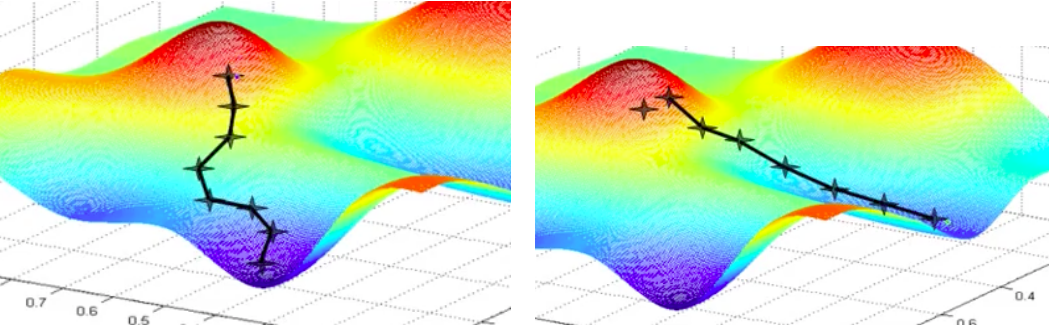
\includegraphics[scale=0.4]{graddesc.png}
  \caption{Two different gradient descent optimizations of the same non-convex function: the slightly different starting points lead to different local minima (from \cite{coursera-ml} video: ``Gradient Descent'').}
  \label{fig:graddesc}
\end{figure}

The explanation so far comprises the intuition behind the ``vanilla'' version of the algorithm, the \textbf{batch gradient descent} (abbreviated {\it BGD}), which is presented in the next subsection. This basic version is exposed to many issues that can drastically alter its performance, and for most complex settings requires some tweaking to be able to perform acceptably. In fact, the different algorithms of the gradient descent family are variations of the {\it BGD} motivated by such issues. Therefore it is desirable to have a sound understanding of the {\it BGD}, in order to be able to identify possible performance issues, understand their cause and identify the most appropiate variation for each case. This will also be covered in the next subsections with some detail.\\

\subsubsection{Batch Gradient Descent}

The general strategy is to start with any convenient parameter vector \(\theta^{(0)}\) and {\it simultaneously} update all its \(\theta_j\) components as follows:
\begin{equation*}
  \begin{aligned}
    & \text{repeat until \(|\theta_j^{\,(i+1)}-\theta_j^{\,(i)}|<\epsilon\):}\\[5mm]
    & \qquad \qquad \theta_j^{\,(i+1)} :=  \theta_j^{\,(i)}-\alpha\frac{\partial J}{\partial\theta^{\,(i)}_j}  \\[3mm]
    & i \in \mathbb{N}, \quad \epsilon, \alpha \in \mathbb{R}^+, \quad \theta  \in \mathbb{R}^{(n)}, \quad  \forall j \in \{1, ...,  n\}
  \end{aligned}
\end{equation*}

\(|\theta_j^{\,(i+1)}-\theta_j^{\,(i)}|<\epsilon\) is the convergence condition: Ideally, it would be sensible to say ``repeat until convergence'' instead, which would imply that \(\epsilon=0\), but in some cases, it may be convenient to stop before this happens. In others, it may be desirable to keep going.\\

The \(\alpha\) factor is called the \textbf{learning rate}, and affects directly the size of each step. As already seen, for non-convex functions the information given by the derivative holds only locally. More precisely, holds only at infinitesimal level: this means that the most precise way to update \(\theta\) would be to have the smallest \(\alpha\) possible, but this would maximize the number of iterations needed in order to converge. On the opposite side, a very big \(\alpha\) would cause the algorithm to go ``too far away'', and the information given by the derivative of \(J\) would become useless (in some cases an oversized learning rate could even make {\it BGD} diverge to the infinity). So in an ideal scenario, it would be possible to apply the optimal \(\alpha\) to each iterative step, but due to the properties of most const functions, there is no trivial systematic way of calculating it. In fact, choosing the appropiate learning rate is one of the key points which the different gradient descent variants focus on.\\

%% Luckily enough, it is possible to know if it is too small or too big (NG VIDEOS ON EVOLUTION CURVES WHEN m PROGRESSES?). It must also be noted that, even with a fixed learning rate, the size of steps will decrease if the gradient itself will become smaller. This can mean, with some luck, that the step size will nicely adapt when converging to a minimum, but could also make some parameters converge into any suboptimal zero-gradient point (e.g. bad local minima, \textbf{local maxima} or \textbf{saddle points}), and stop there. It is possible to overcome, or at least mitigate some of this issues by applying MOMENTUM to the vector, and SECOND, THIRD ORDER?? (hessian, jacobian) derivatives. Other gradient descent variations explained here will as well focus on this techniques.\\
%% regarding momentum: \url{http://distill.pub/2017/momentum/}

And last but definitely not least, there is a performance problem: every cost function, as well as any of its derivatives, is based on a given dataset, and requires to perform calculations for every given sample. On the top of that, BGD does this for every feature, once per iteration! (hence the ``batch'' term). So given m samples, j features and i total steps until convergence, the worst-case amount of operations will be BGD=O(m*j*i), which scalates very poorly. There are GD variations that overcome this problem, as explained further on. (vectorization, parallel GD, SGD, miniBatchGD, early stopping)\\



\subsubsection{Stochastic and Minibatch Gradient Descent}

``Stochastic gradient descent has many important uses outside the context of deep learning. It is the main way to train large linear models on very large datasets. For a fixed model size, the cost per SGD update does not depend on the training set size m. In practice, we often use a larger model as the training set size increases, but we are not forced to do so. The number of updates required to reach convergence usually increases with training set size. However, as m approaches infinity, the model will eventually converge to its best possible test error before SGD has sampled every example in the training set. Increasing m further will not extend the amount of training time needed to reach the model’s best possible test error. From this point of view, one can argue that the asymptotic cost of training a model with SGD is O(1) as a function of m''\cite[p.152]{goodfellow}

Again, starting with any convenient parameter vector \(\theta^{(0)}\) and {\it simultaneously} updating all its \(\theta_j\) components:
\begin{equation*}
  \begin{aligned}
    & m \in \mathbb{N}\;\hat{=} \text{ dataset size}\\
    & b \in \mathbb{N}\;\hat{=} \text{ batch size, } b\leq m\\
    & I \in \mathbb{N}\;\hat{=} \text{ number of iterations}\\[5mm]
    & \text{1) shuffle all } (X^{(i)}, y^{(i)}) \text{ tuples in the dataset}\\[2mm]
    & \text{2) for } i \in \{1, ..., I\} \text{:}\\[5mm]
    & \qquad \qquad j := (b*i)(mod\;m)\\
    & \qquad \qquad \theta^{\,(i+1)} :=  \theta^{\,(i)}-\frac{\alpha}{b}\frac{\partial}{\partial\theta^{\,(i)}}J(\theta, X^{(j...(j+b))}, y^{(j...(j+b))})  \\[3mm]
    & \alpha \in \mathbb{R}^+, \quad \theta  \in \mathbb{R}^{(n)}, \quad  \forall j \in \{1, ...,  n\}
  \end{aligned}
\end{equation*}


\subsubsection{Further Optimizations}

One of the problems that poses the use of gradient descent, is the application of a proper learning rate. This issue becomes even bigger in the stochastic gradient descent algorithm, which features also further hyperparameters like the batch size. Algorithms like the Adam optimizer\cite{adam} offer a solution to this problem by taking into account further derivatives of the cost function (the so-called Hessian and Jacobian matrices) in order to calculate a dynamic, context-depending learning rate.



%%    \subsection{Overfitting and Regularization}\label{regularization}

%% http://neuralnetworksanddeeplearning.com/chap3.html

%%   reminder: the derivative of L2 \(\lambda* 0.5 * \Theta\) with respect to theta a,b is lambda* theta a,b

%%    FIGURES:
%%    in log.reg., comparative graph showing effects of regularization: no reg, ok reg, high reg



%%    When a model tends to oversimplify his hypothesis, we say it is \textbf{biased}. And conversely, if due to its excesive capacity tends to memorize the training data thus failing to generalize, we say it is \textbf{overfitting} the data. A more intuitive vision is given by the {\it skinny jeans} approach\cite{stretchpants}: finding the model that fits perfectly (the skinny jeans) is very hard, so everybody end up wearing loose pants (overfitting). The solution for that are the stretchpants (regularizing): ``they fit well, but because they're flexible, they don't make things harder to fit in''. Thus, \textbf{``regularizing means applying artificial constraints on your network, that implicitly reduce the number of free parameters, while not making it more difficult to optimize''}.

%%    -early termination still the best way

%%    In his
%%    l2 and dropout regul. overfitting and bias

%%    normal equations:  (see \url{https://en.wikipedia.org/wiki/Regularization_(mathematics)#Tikhonov_regularized_least_squares}).

%%    \subsection{Cross Validation}\label{crossvalidation}
%%    FIGURES: learning curves for bias, overfitting and ok
%%    In supervised learning, the problem formulation talks about a training set. Apart from the considerations in\ref{datapreprocessing}, the bigger it is, better for the system
%%    cross validation set, learning curves

%%    higher-order CV procedures: auto-weka (2016): \url{http://www.cs.ubc.ca/labs/beta/Projects/autoweka/}
%%    \subsection{Error Metrics}\label{errormetrics}
%%    precision recall f2
%%    en logreg,hablar de cambiar el threshold para variar el prec y recall

%% voting


%%         TALK ABOUT AUC ROC?



\subsection{KL-Divergence and Cross-Entropy}\label{kldivergence}

The cross-entropy is used to measure the similarity between the hypothesis and the dataset in classification problems, modelled as probability distributions. To become a better idea on how does this work, some background on information theory is needed. Specifically, how to quantify the information given by a probability distribution. Most of the explanations of this section (especially the quotes), as well as extra information can be found in \cite[p.73]{goodfellow}.
\subsubsection{Self-Information and Shannon entropy}

The information of an event \(\epsilon_{ic} := \{Y_i=c\}\) given by any probability distribution \(P(Y)\) is related, among other things described in \cite[p.73]{goodfellow}, to the likelihood of that event: ``learning that an unlikely event has occurred is more informative than learning that a likely event has occurred''. It can be quantified with the {\it self-information} of such event:
\begin{equation*}
  I(\epsilon_{ic}) = -log(P(\epsilon_{ic}))\\[3mm]
\end{equation*}
If the basis of the logarithm is 2, the returned value is the amount of information in {\it bits}. If the natural logarithm (with basis \(e\)) is used, the information unity are the {\it nats}: ``One nat is the amount of information gained by observing an event of probability \(e^{-1}\)''\cite[p.73]{goodfellow}. This way it is also possible to quantify the average amount of information in the whole distribution by calculating the expectation for the self-information over all its possible outcomes. This is known as the {\it Shannon entropy} of the variable, expressed here in its version for discrete probability distributions:
\begin{equation*}
  H(P) = \mathbb{E}_P[I(Y)] =  \sum_{i=1}^{m} \Big\{P(\epsilon_{ic}) I(\epsilon_{ic}) \Big\} =  - \sum_{i=1}^{m} \Big\{P(\epsilon_{ic}) log(P(\epsilon_{ic})) \Big\}\\[3mm]
\end{equation*}

When used with basis 2, this calculation ``gives a lower bound on the number of bits needed on average to encode symbols drawn from a distribution \(P\). Distributions that are nearly deterministic (where the outcome is nearly certain) have low entropy; distributions that are closer to uniform have high entropy''.

\subsubsection{KL-Divergence}
``If we have two separate probability distributions \(P(Y)\) and \(Q(Y)\) over the same random variable Y, we can measure how different these two distributions are using the Kullback-Leibler (KL) divergence'':
\begin{equation*}
  D_{KL}(P || Q) = \mathbb{E}_P[log(P(Y))-log(Q(Y))] = \sum_{i=1}^{m} \Big\{P(\epsilon_{ic}) (log(P(\epsilon_{ic}))-log(Q(\epsilon_{ic})) \Big\}\\[3mm]
\end{equation*}

The KL-divergence is non-negative, and zero if and only if both distributions are identical. For this reason ``it is often conceptualized as measuring some sort of distance between these distributions. However, it is not a true distance measure because it is not symmetric''. There are some caveats (especially the fact that it is not a symmetric operation, and others explained in \cite[p.74]{goodfellow}), but the idea of measuring the distance between two distributions will suffice for the present explanation.

\subsubsection{Cross-Entropy and Intuition}
When training a classificator, the information of the dataset as a probabiliy distribution can be purely regarded in terms of the information contained in its labels. Conversely, the hypothesis of the model can be also regarded as a different distribution, generating a different set of labels. This way, the KL-Divergence can be systematically used to measure how well does the hypothesis resemble the training data, regardless of the specific features of the data space. In that case, the optimization objective is to minimize it, which can be done with gradient descent. This is precisely the strategy followed by unsupervised learning algorithms like t-SNE\cite{t-sne}.\\

But, when performing supervised learning, only the distribution given by the hypothesis is optimized, so it is not necessary to take both \(log(P(Y))\) and \(log(Q(Y))\) terms into account. This is where the cross-entropy comes into play:

\begin{equation*}
  \mathcal{L}(P, Q) = -\mathbb{E}_P[log(Q(Y))] = -\sum_{i=1}^{m} \Big\{P(\epsilon_{ic}) log(Q(\epsilon_{ic})) \Big\}\\[3mm]
\end{equation*}

In other words, ``minimizing the cross-entropy with respect to Q is equivalent to minimizing the KL divergence, because Q does not participate in the omitted term''\cite[p.75]{goodfellow}. An explanation on how to use it in combination with the softmax function to perform gradient descent optimization can be found in \ref{logregcost}.

%% \subsection{Robust Models}\label{robust}

%%       Applying the same cost function to every sample and taking the overall average causes the model to be sensitive to noisy and context-dependent data. For example, hardware errors and other excepcionalities may generate samples way out from the context, greatly incrementing the output of the cost function, thus affecting the learning process. Robust regression methods (as, for example, the {\it Theil-Sen estimator}, see \cite{theil} and \cite{sen}) incorporate extra criteria to define a \textbf{prior} context in which data is expected to happen, and properly handle such cases in which out-of-context samples, known as \textbf{outliers} may skew the result. As for 2017, wikipedia warns\cite{robust-wiki} that such methods are surprisingly unpopular:

%% \begin{quote}
%% Despite their superior performance over least squares estimation in many situations, robust methods for regression are still not widely used. Several reasons may help explain their unpopularity (Hampel et al. 1986, 2005). One possible reason is that there are several competing methods and the field got off to many false starts. Also, computation of robust estimates is much more computationally intensive than least squares estimation; in recent years however, this objection has become less relevant as computing power has increased greatly. Another reason may be that some popular statistical software packages failed to implement the methods (Stromberg, 2004). The belief of many statisticians that classical methods are robust may be another reason.
%% \end{quote}

%% And indeed, the fact that such ``bibles'' as \cite{russell}, \cite{bishop} or \cite{goodfellow} do not contain a single reference to the term is a strong indicator of that. Regarding this thesis, as already explained in the beginning of this chapter, it is assumed that the dataset is comprehensive and correctly labeled and therefore no robust methods will be needed. For this reason, they won't be further covered (see \cite{andersen} and \cite{tendeiro} for a broad coverage on the topic).


%% \subsection{Non-parametric Models}\label{nonparametric}

%%                            REVISE THIS! quote ``all of statistics'' for definition of NPM. Also talk briefly about KNN (see goodfellow p. 143) because the 2015 paper uses it. \cite{svm_knn}

%%         All the models explained so far are parametric, meaning that they have a fixed set of parameters independently of how does the data look like. This forces the model to make some assumptions on the data and its context, which has advantages and disadvantages. Non-parametric models adapt their architecture to the given dataset, which implies a totally different workflow, in which the data itself directly influences many design decisions. For this reason, this approach is known as {\it data-driven} design (as opposed to the {\it model-driven} approach associated with parametric models).\\
%%         Both approaches are legitimate and useful depending on the context. Currently, parametric models are gathering the most attention. The reasons for that are that, in the best-case scenario,  having a fixed set of parameters and their combinations can lead to an explicit interpretation on how does the ``ground truth'' work, which can help to transfer the achieved knowledge to other domains and applications more easily. Plus, because of their more predictable architecture, it is possible to achieve a better sinergy amongst the different components (especially libraries and hardware) and effectively scale them up.\\
%%         Of course, the best-case scenario for parametric models doesn't always apply, and some problem domains can be tackled more effectively following a {\it data-driven} approach. Non-parametric models are in any case a field of expertise on their own and won't be covered here since they didn't play a relevant role in this thesis. Some examples of non-parametric models are: {\it pieceweise linear nonparametric regression} (a.k.a. ``connect-the-dots''), {\it \(k\)-nearest neighbours average}, {\it \(k\)-nearest neighbours regression} and {\it locally weighted regression}.

%% \subsection{Universal Approximation Theorem}
%% asdf

%% %% \subsection{Central Limit Theorem?}
%% %% asdf

%% %% \subsection{Manifolds}
%% %% fdas

%% \subsection{Invariance}
%% fdas

%% \subsection{Sparsity and Parameter Sharing}
%% \url{http://ml.typepad.com/machine_learning_thoughts/2005/11/when_does_spars.html}
